\scanpage{109}
Plus précisément, si $\underline t_0\inserted{=\{a,b,c\}}$ est un triangle de sommet $a$ ne contenant ni $s$ ni $t$ (il y en a par l'hyp. que $c\neq1$ i.e. $c\geq2$), on peut choisir de plus $u$ (i.e. $\underline t,\unsure{\underline t'|\underline\tau}$) tel que \deleted{$ua=a,\ ub=c,\ uc=b$} \inserted{$u\mid\underline t_0=\mathrm{id}_{\underline t_0}$ (i.e., $ua=a,\ ub=b,\ uc=c$} \deleted{\unsure{$b,c$} et $ua=a,\ ub=c,\ uc=b$.}

\figure{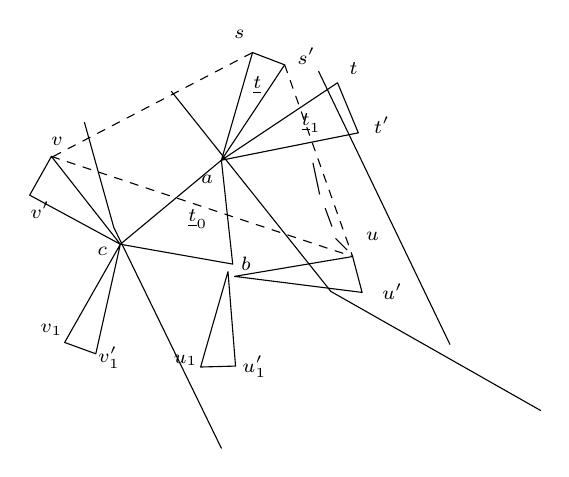
\begin{tikzpicture}[x=0.012cm,y=-0.012cm,line cap=round,line join=round]
\draw (233,394)--(126,483)--(245,504)--cycle;
\draw (233,394)--(266,280)--(300,293)--cycle;
\draw (233,394)--(356,312)--(378,365)--cycle;
\draw (126,483)--(53,390)--(30,431)--cycle;
\draw (126,483)--(67,587)--(100,599)--cycle;
\draw (240,512)--(211,613)--(248,612)--cycle;
\draw (247,517)--(372,496)--(382,534)--cycle;
\draw (330,397)--(337,430);
\draw (343,445)--(350,464);
\draw (354,477)--(366,489);
\draw (88,354)--(119,465)--(233,699);
\draw (180,321)--(349,533)--(571,659);
\draw (336,300)--(475,589);

\node[inner sep=1pt,font=\scriptsize] at (218,414) {$a$};
\node[inner sep=1pt,font=\scriptsize] at (259,504) {$b$};
\node[inner sep=1pt,font=\scriptsize] at (107,490) {$c$};
\node[inner sep=1pt,font=\scriptsize] at (208,456) {$\underline t_0$};
\node[inner sep=1pt,font=\scriptsize] at (252,261) {$s$};
\node[inner sep=1pt,font=\scriptsize] at (323,284) {$s'$};
\node[inner sep=1pt,font=\scriptsize] at (271,315) {$\underline t$};
\node[inner sep=1pt,font=\scriptsize] at (373,297) {$t$};
\node[inner sep=1pt,font=\scriptsize] at (403,357) {$t'$};
\node[inner sep=1pt,font=\scriptsize] at (328,355) {$\underline t_1$};
\node[inner sep=1pt,font=\scriptsize] at (59,374) {$v$};
\node[inner sep=1pt,font=\scriptsize] at (41,447) {$v'$};
\node[inner sep=1pt,font=\scriptsize] at (393,475) {$u$};
\node[inner sep=1pt,font=\scriptsize] at (414,533) {$u'$};
\node[inner sep=1pt,font=\scriptsize] at (53,574) {$v_1$};
\node[inner sep=1pt,font=\scriptsize] at (114,603) {$v'_1$};
\node[inner sep=1pt,font=\scriptsize] at (195,606) {$u_1$};
\node[inner sep=1pt,font=\scriptsize] at (268,613) {$u'_1$};
\draw[dashed] (55,390)--(266,280);
\draw[dashed] (300,293)--(372,496);
\draw[dashed] (53,390)--(372,496);
\end{tikzpicture}}

\deleted{\unsure{Théor.} \unsure{Variante|Nouveau} On peut trouver $v\in G^0$ tel que $v\mid\underline t_0=\underline t_0$ ($va=a,vb=b,vc=c$) et $vs=t$}

\deleted{\uline{\unsure{Récette|Recette}} On \deleted{choisit $u$ lié à $t$ et $s$} complète les triangles $\underline t=\{a,s,s'\}$ et $\underline t_0=\{a,b,c\}$ (par $s'$ et $c$). \unsure{On} \deleted{\unsure{pour} $\unsure{\underline t=} $} a donc $\widetilde{\underline E}_a,\widetilde E_b,\widetilde{\underline E}_c$ etc \ldots) on choisit \textcircled{$u$} \inserted{$\neq a$} lié à $b$ et à $s$ i.e. $u\in\widetilde E_b$ lié à $s$, on complète en triangle $\{s,u,v\}$ sur $(a,b,c)$, donc}

\figure{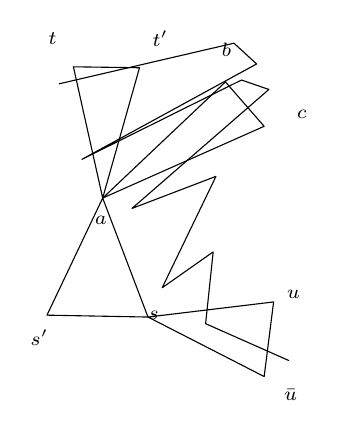
\begin{tikzpicture}[x=0.012cm,y=-0.012cm,line cap=round,line join=round]
\draw (156,1044)--(125,905)--(195,906)--cycle;
\draw (156,1044)--(286,921)--(327,968)--cycle;
\draw (156,1044)--(97,1168)--(204,1170)--cycle;
\draw (204,1170)--(337,1154)--(327,1233)--cycle;
\draw (110,923)--(295,880)--(319,902)--(134,1003)--(303,919)--(332,929)--(187,1055)--(276,1021)--(219,1139)--(273,1101)--(265,1177)--(353,1216);

\node[inner sep=1pt,font=\scriptsize] at (103,875) {$t$};
\node[inner sep=1pt,font=\scriptsize] at (217,875) {$t'$};
\node[inner sep=1pt,font=\scriptsize] at (287,887) {$b$};
\node[inner sep=1pt,font=\scriptsize] at (367,955) {$c$};
\node[inner sep=1pt,font=\scriptsize] at (154,1068) {$a$};
\node[inner sep=1pt,font=\scriptsize] at (89,1192) {$s'$};
\node[inner sep=1pt,font=\scriptsize] at (210,1168) {$\unsure{s}$};
\node[inner sep=1pt,font=\scriptsize] at (358,1146) {$u$};
\node[inner sep=1pt,font=\scriptsize] at (355,1252) {$\bar u$};
\end{tikzpicture}}

\[
\deleted{\begin{aligned}
u\in\widetilde E_b,\ v\in\widetilde E_c &\qquad \{s,u,v\}\in\widetilde T\subset T\\
u'\in\widetilde E_b,\ v'\in\widetilde E_c &\qquad (s',u',v')\in\widetilde T\subset T
\end{aligned}}
\]

\deleted{d'où}

\[ \deleted{\left[\begin{aligned}(b,u,u')&\in T\\(c,v,v')&\in T\end{aligned}\right]} \]

\deleted{\deleted{On \unsure{prend|peut} choisit} Quitte à échanger $t,t'$ \unsure{O.P.S} $t$ lié à $u$, \deleted{\unsure{$t=$}} complétons alors en le triangle}

\[ \deleted{(t,u,\underset{\substack{\unsure{\rotatebox{-90}{$\in$}|\uparrow}\\ \widetilde E_c}}{v_1})\in\widetilde T} \]

\deleted{Alors $t'$ est lié à $u'$, donc pas à $v'$, donc à $v$ et complétons $(t',v)$ en triangle}

\[ \deleted{(t',v,\underset{\substack{\unsure{\rotatebox{-90}{$\in$}|\uparrow}\\ \widetilde E_b}}{u_1})\in\widetilde T\subset T} \]

\deleted{Et avec $u_1,v_1$ on a aussi}

\[ \deleted{u'_1\in\widetilde E_b,\quad v'_1\in\widetilde E_c\qquad \{b,u_1,u'_1\},\ \{c,v_1,v'_1\}\in T} \]

% archive sheet number: 108
